% =====================================================================
% DBA - Proyecto final - Entrega 2
% Límites PDET: carga en MongoDB e índices espaciales
% =====================================================================
\documentclass[11pt,a4paper]{article}
% =====================================================================
% Preámbulo compartido - DBA Proyecto final
% =====================================================================
\usepackage[utf8]{inputenc}
\usepackage[T1]{fontenc}
\IfFileExists{lmodern.sty}{\usepackage{lmodern}}{}
\usepackage[spanish,es-noshorthands,es-tabla]{babel}
\usepackage[margin=2.5cm]{geometry}
\usepackage{amsmath,amssymb}
\usepackage{booktabs,tabularx,array}
\usepackage{enumitem}
\usepackage[dvipsnames,table]{xcolor}
\usepackage{graphicx}
\usepackage{tikz}
\usetikzlibrary{calc,positioning}
\usepackage{listings}
\usepackage{caption}
\usepackage{float}
\usepackage[hidelinks]{hyperref}
\usepackage{xurl}

% --- Colores --------------------------------------------------------
\definecolor{acento}{HTML}{2F6FDB}
\definecolor{gris}{HTML}{6B6B6B}
\hypersetup{colorlinks=true, linkcolor=acento, urlcolor=acento, citecolor=acento}

% --- Tablas ---------------------------------------------------------
\newcolumntype{L}{>{\raggedright\arraybackslash}X}
\renewcommand{\arraystretch}{1.25}

% --- Listas ---------------------------------------------------------
\setlist{itemsep=2pt, topsep=4pt}

% --- Código (JSON / mongosh) ----------------------------------------
\lstdefinestyle{codigo}{
  basicstyle=\ttfamily\footnotesize,
  breaklines=true,
  columns=fullflexible,
  keepspaces=true,
  frame=single,
  framerule=0.3pt,
  rulecolor=\color{gray!50},
  backgroundcolor=\color{gray!6},
  xleftmargin=4pt, xrightmargin=4pt,
  showstringspaces=false,
  literate={á}{{\'a}}1 {é}{{\'e}}1 {í}{{\'i}}1 {ó}{{\'o}}1 {ú}{{\'u}}1
           {Á}{{\'A}}1 {É}{{\'E}}1 {Í}{{\'I}}1 {Ó}{{\'O}}1 {Ú}{{\'U}}1
           {ñ}{{\~n}}1 {Ñ}{{\~N}}1
}
\lstset{style=codigo}

% --- Atajos ---------------------------------------------------------
\newcommand{\campo}[1]{\texttt{#1}}
\newcommand{\pendiente}[1]{\textcolor{gris}{\textit{[Pendiente -- #1]}}}

\begin{document}

% ------------------------------- Portada -----------------------------
\begin{titlepage}
  \centering
  {\large Pontificia Universidad Javeriana\par}
  {\large Departamento de Ingeniería de Sistemas\par}
  \vspace{0.8cm}
  {\large Administración de Bases de Datos (DBA) -- 2026-30\par}
  \vspace{2.5cm}
  {\Huge\bfseries Proyecto final\par}
  \vspace{1cm}
  {\LARGE Entrega 2: Límites PDET -- carga en MongoDB\\ e índices espaciales\par}
  \vspace{1cm}
  {\large Potencial solar en techos de los municipios PDET\par}
  \vspace{3cm}
  {\large
    Maria Camila Beltran \\
    \vspace{0.5cm}
    Jorge Fortich \\
    \vspace{0.5cm}
    Jose Eduardo Valeriano \\
    \vspace{0.5cm}
    Samuel Osorio Rodríguez\par}
  \vspace{3cm}
  {\large Profesor: Andrés Oswaldo Calderón Romero, Ph.D.\par}
  \vspace{3cm}
  {\large \pendiente{fecha de entrega}\par}
\end{titlepage}

\tableofcontents
\newpage

% =====================================================================
% 1. Contexto
% =====================================================================
\section{Contexto}
\label{sec:contexto}

Esta entrega corresponde a la \textbf{semana 2} del plan de implementación
definido en la Entrega 1 (sección~3): cargar los límites de los 170
municipios PDET en MongoDB y dejar evidencia del índice espacial que soporta
las consultas sobre ellos. El diseño del esquema, el diagrama E-R y el
diccionario de datos no cambian respecto a la Entrega 1 y no se repiten aquí;
se referencian cuando hace falta.

El flujo de esta semana tiene cuatro pasos encadenados por
\campo{src/municipios/run.py} (lo que corre \campo{make municipios}):
descargar el MGN 2025, cruzarlo con \campo{MunicipiosPDET.xlsx}, validar y
reparar las geometrías, y finalmente crear las colecciones, cargarlas e
indexarlas en MongoDB. 
% =====================================================================
% 2. Descarga y cruce con PDET (Jorge)
% =====================================================================
\section{Descarga del MGN y cruce con PDET}
\label{sec:descarga}


% =====================================================================
% 3. Validación, reparación y reproyección (Maria Camila)
% =====================================================================
\section{Validación, reparación y reproyección de geometrías}
\label{sec:geometria}


% =====================================================================
% 4. Esquema, carga e índices (Samuel)
% =====================================================================
\section{Esquema, carga e índices en MongoDB}
\label{sec:samuel}

Esta sección cubre las cuatro partes:
\campo{schema.py}, \campo{carga.py}, \campo{indices.py} y
\campo{evidencia.py}. El código completo está en
\campo{src/municipios/}; aquí se explica qué hace cada uno y se muestra
evidencia de que funciona contra una base MongoDB real.

\subsection{Colecciones con validación \texorpdfstring{\campo{\$jsonSchema}}{\$jsonSchema}}
\label{sec:samuel-schema}

\campo{schema.py} crea \campo{municipios} y \campo{fuentes} con un validador
\campo{\$jsonSchema} derivado directamente del diccionario de datos de la
Entrega 1 (sección 5): campos requeridos, tipos BSON y, para
\campo{subregion\_pdet} y \campo{calidad}, la forma exacta de los
subdocumentos embebidos. Si la colección ya existe (por ejemplo al volver a
correr \campo{make schema}), usa \campo{collMod} en vez de
\campo{create\_collection} para no fallar.

\begin{figure}[H]
  \centering
  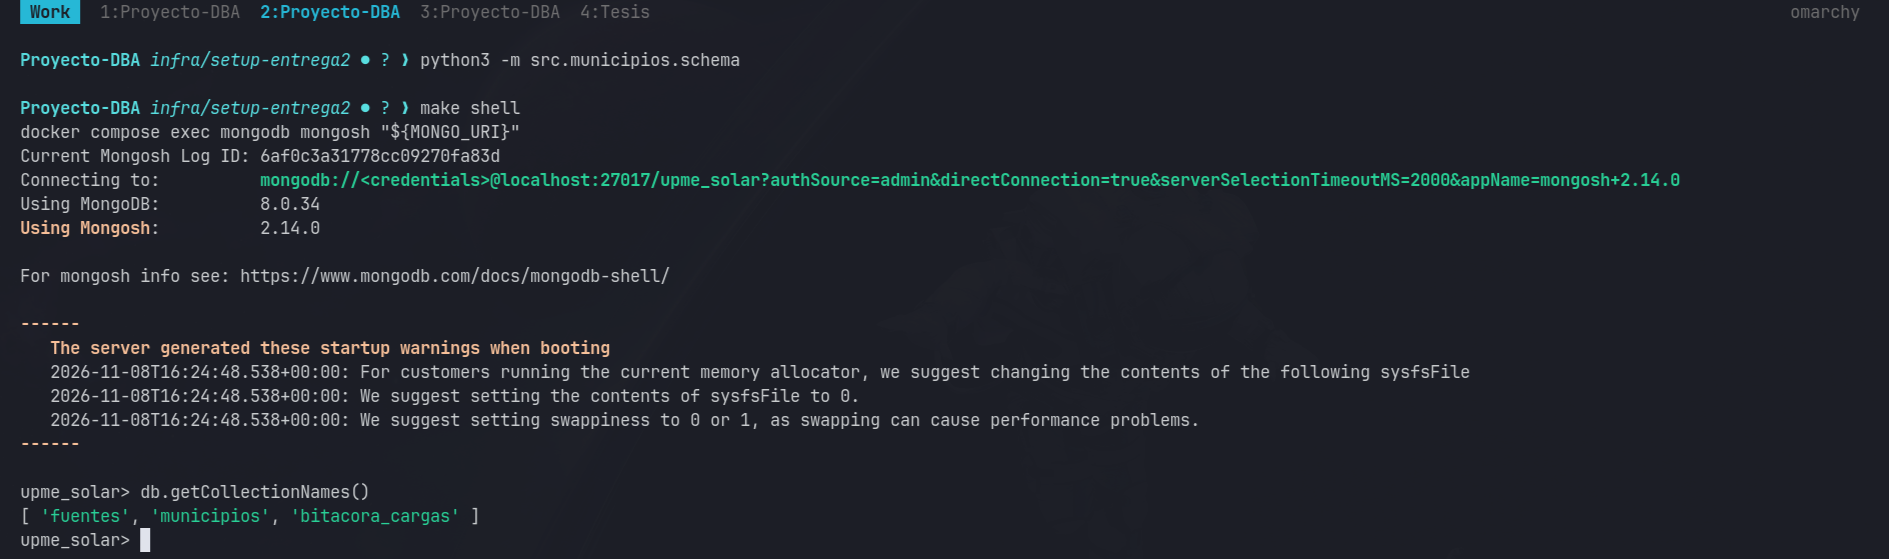
\includegraphics[width=\textwidth]{img/cap_schema.png}
  \caption{Ejecución de \campo{schema.py}: crea ambas colecciones sin errores.}
  \label{fig:cap-schema}
\end{figure}

Como evidencia de que el validador realmente se aplica, se intentó insertar
un documento incompleto directamente por \campo{mongosh}: MongoDB lo rechaza
con el código de error 121 y lista los campos que faltan.

\begin{figure}[H]
  \centering
  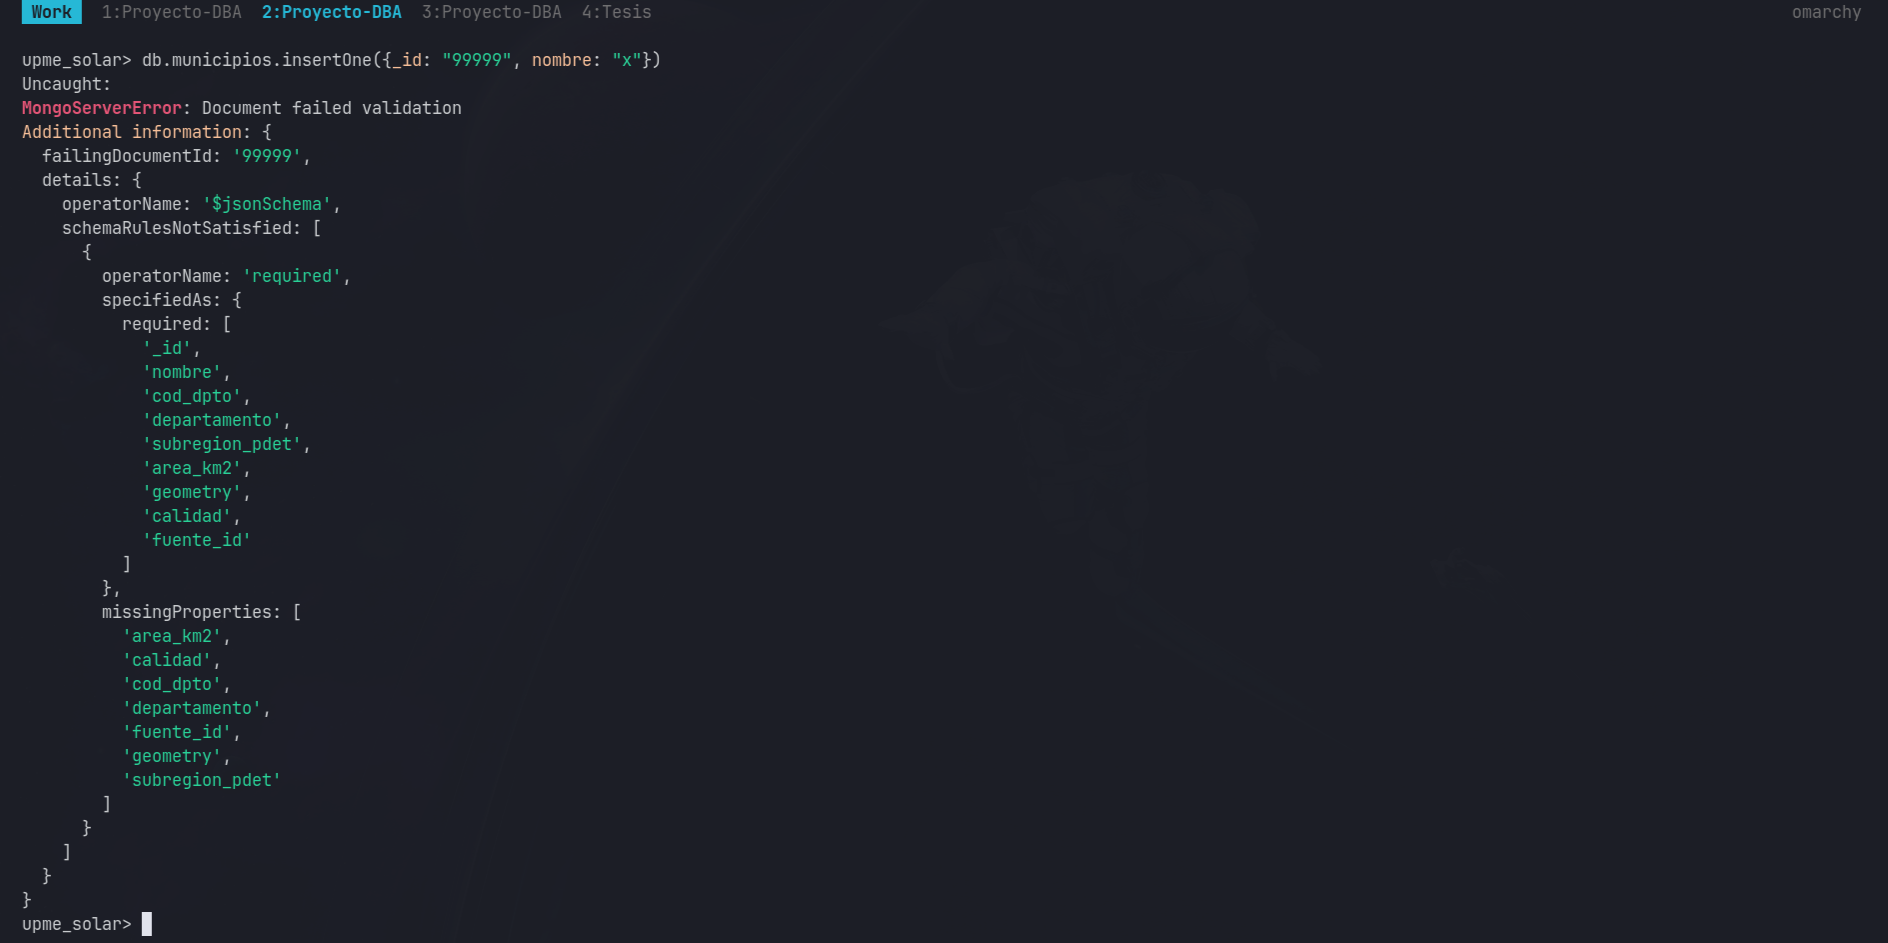
\includegraphics[width=\textwidth]{img/cap_validacion.png}
  \caption{Un documento sin los campos obligatorios es rechazado por el
  validador \campo{\$jsonSchema}.}
  \label{fig:cap-validacion}
\end{figure}

\
% =====================================================================
% 5. Mapa y control de calidad (Jose Eduardo)
% =====================================================================
\section{Mapa de control y chequeo de calidad}
\label{sec:mapa}



% =====================================================================
% 6. Conclusiones y próximos pasos
% =====================================================================
\section{Conclusiones y próximos pasos}
\label{sec:conclusiones}



\end{document}
